
\begin{savequote}[75mm] 
Một hệ thống cơ sở dữ liệu tốt là nền tảng cho sức mạnh kinh doanh.
\qauthor{Dữ liệu là tài sản} 
\end{savequote}

\chapter{Giới thiệu}

\newthought{Hệ thống cơ sở dữ liệu} là một phần quan trọng trong các ứng dụng e-commerce hiện đại. Hệ thống này cho phép lưu trữ, quản lý và truy vấn lượng lớn dữ liệu một cách hiệu quả. Một thiết kế cơ sở dữ liệu tốt sẽ cải thiện hiệu suất của hệ thống, giảm chi phí vận hành và nâng cao trải nghiệm người dùng.
$$\zeta = \frac{1039}{\pi}$$


For an example of a full page figure, see Fig.~\ref{fig:myFullPageFigure}.

\section{This is section one}

\blindtext


\blindtext


\begin{figure}  
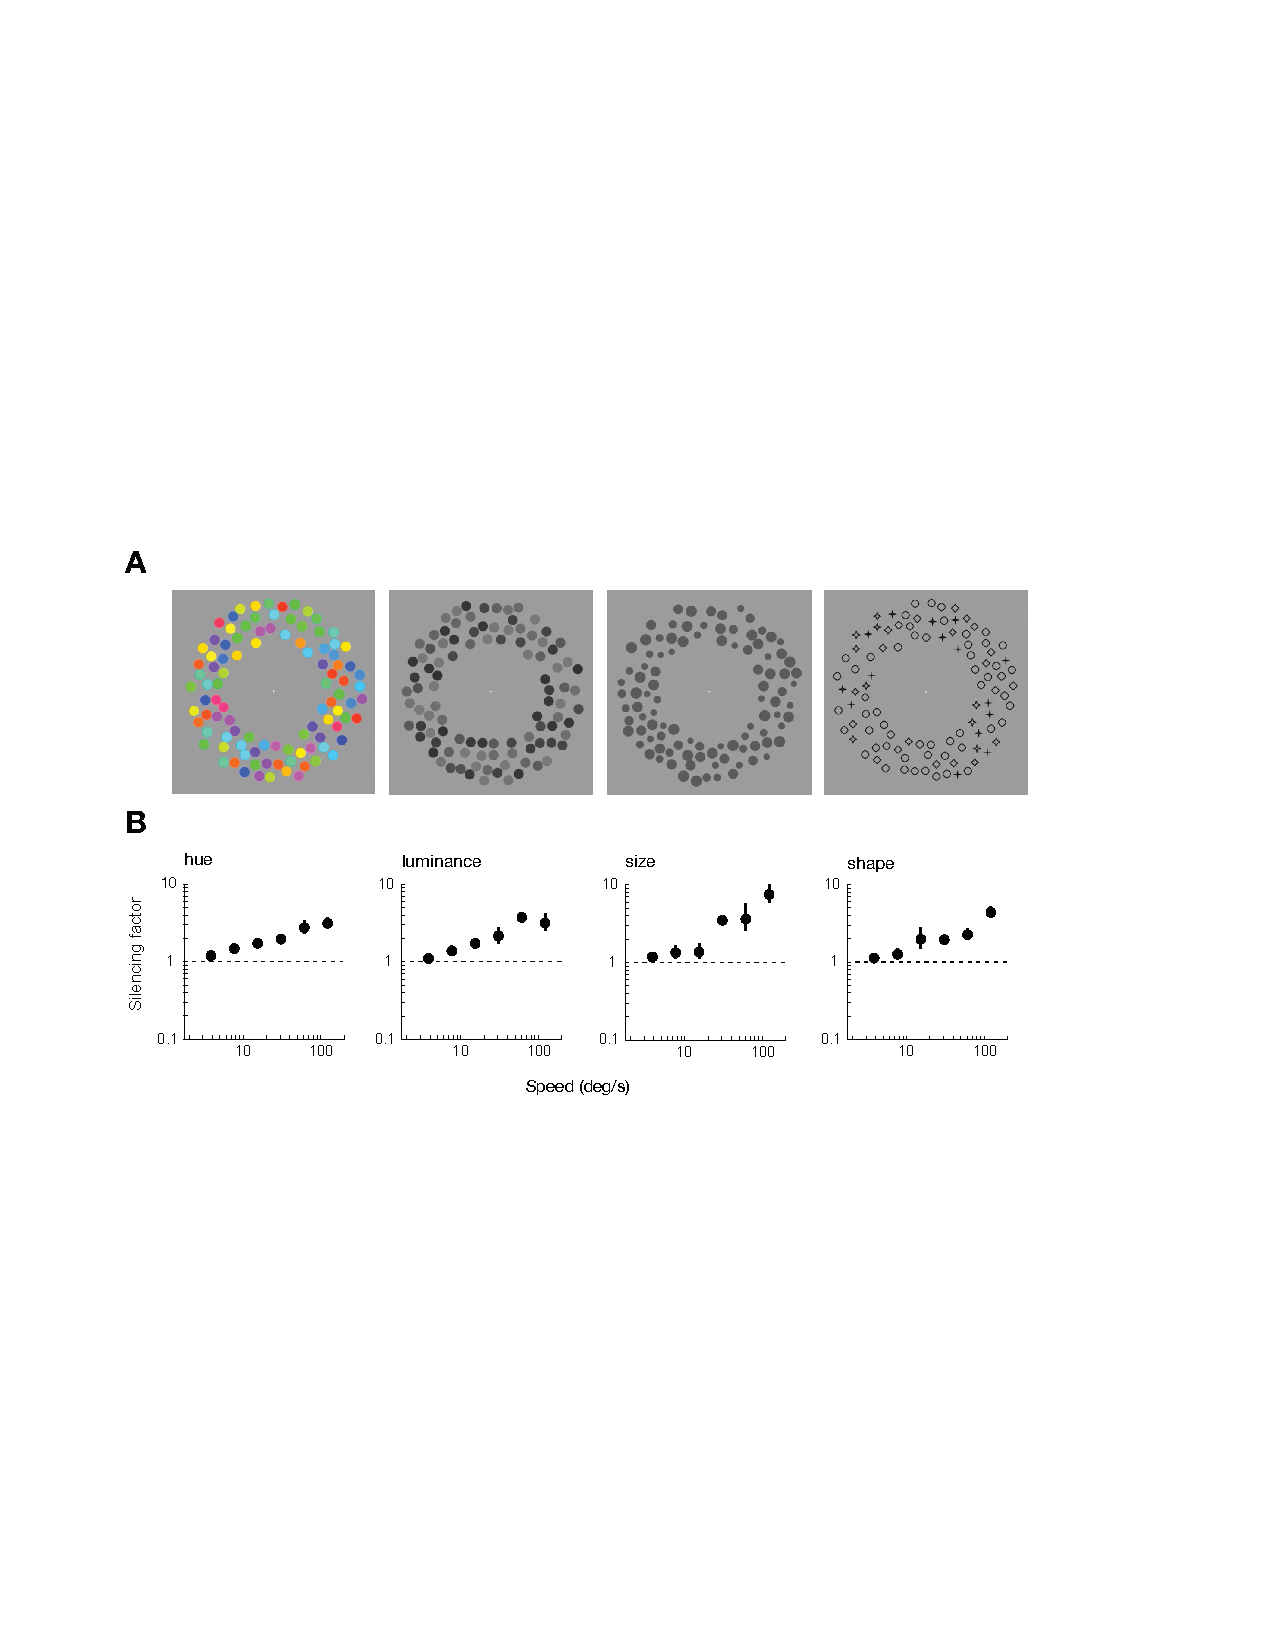
\includegraphics[width=\textwidth]{figures/fig1}
\caption[Short figure name.]{This is a figure that floats inline and here is its caption.
\label{fig:myInlineFigure}}
\end{figure}

\blindtext

\begin{figure}  
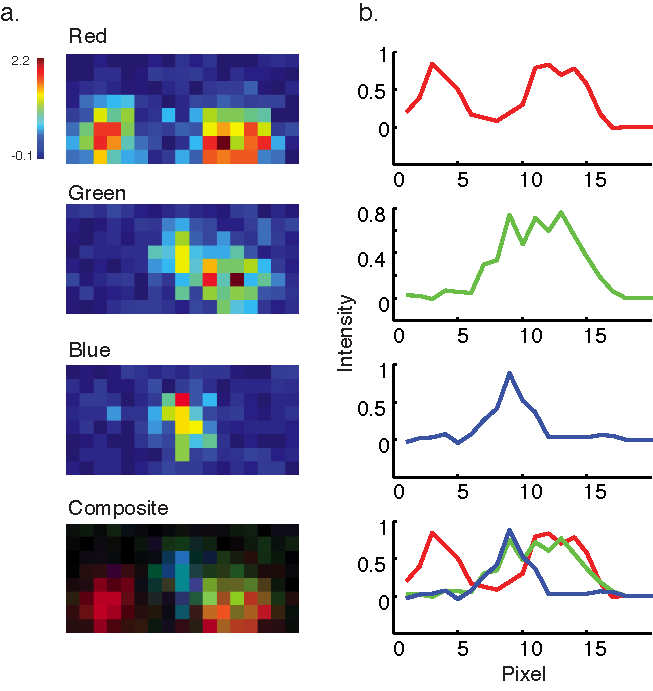
\includegraphics[width=\textwidth]{figures/fullpage}
\caption[Short figure name.]{This is a full page figure using the FPfigure command. It takes up the whole page and the caption appears on the preceding page. Its useful for large figures. Harvard's rules about full page figures are tricky, but you don't have to worry about it because we took care of it for you. For example, the full figure is supposed to have a title in the same style as the caption but without the actual caption. The caption is supposed to appear alone on the preceding page with no other text. You do't have to worry about any of that. We have modified the fltpage package to make it work. This is a lengthy caption and it clearly would not fit on the same page as the figure. Note that you should only use the FPfigure command in instances where the figure really is too large. If the figure is small enough to fit by the caption than it does not produce the desired effect. Good luck with your thesis. I have to keep writing this to make the caption really long. LaTex is a lot of fun. You will enjoy working with it. Good luck on your post doctoral life! I am looking forward to mine. \label{fig:myFullPageFigure}}
\end{figure}
\afterpage{\clearpage}

\blindtext

\section{This is section two}
\blindtext
\blindmathpaper

\section{This is section three}
\blindtext
\blindmathpaper